{
{\sffamily Her præsenteres forslag til forbedringer til vores
implementation og analyse. Nogle af forslagene kan dog overlappe.
}

\subsection{Generelle forbedringer}
\begin{itemize}
    \item \textbf{Køre analyse på et andet datasæt, som havde større diversitet}\\
        Det kunne være interessant, at sammenligne resultater fra en
        analyse på et andet datasæt. Dette vil give os en indikation på
        om vores resultater fra det oprindelige datasæt kan bruges.
        Ydermere, ville det være interessante, at sammensætte et datasæt
        af malerier, hvor det er et faktum, at de er opbygget efter det
        gyldne snit, med det formål at afprøve metoderne på dette.
    \item \textbf{Implementere programmet i et andet sprog}\\
        For en hurtigere analyse af malerier, kunne programmet
        implementeres i $\textrm{C}^{++}$, som \emph{OpenCV} er
        implementeret i. Programmet kunne med fordel parallelliseres.
\end{itemize}

\subsection{Vurdering af regioner}
\begin{itemize}
    \item \textbf{Sammensmeltning af naiv og udvidet løsning}\\
        Kombinere den naive og udvidede vurdering af regioner, således
        at både regioner der ligger op ad snittet og dem der ligger på
        snittet udvælges. Man kan således også få gjort selve den naive
        vurdering mere sofistikeret, ved også at kigge på regionens
        udstrækning.
    \item \textbf{Pointscore i stedet for binær klassifikation}\\
        Dette vil forkaste den binære klassifikation og i stedet give et
        mere præcist mål for, hvorvidt en region ligger i snittet.  Vi
        har allerede givet et forslag til en sådan metode, hvor man kan
        bruge et topografisk kort, til at udregne omkostninger for
        regioner.  Regionen kunne approksimeres ved brug af et gitter
        eller dennes konvekse hylster.
    \item \textbf{Bonus for regioner, som ligger i flere gyldne snit}\\
        Det kunne være interessant at undersøge, om fundne regioner
        kvalificerer sig til at ligge i mere end et gyldent snit. Med
        den nuværende udtrækning \emph{vil} vi have, at hvis en region
        ligger i to snit, så \emph{vil} denne blive trukket ud to gange.
        Vi vil derfor have brug for metoder til at undersøge, om to
        regioner egentlig er den samme. Dette skal løses med en anden
        metode for udtrækning af regioner. Ved binær klassificering skal
        det overvejes hvordan sådanne regioner belønnes. Bruges der i
        stedet pointscore, vil regionens værdi afspejle dennes specielle
        placering.
    \item \textbf{Ligger der interessante regioner i ``Eye of God''?}\\
        Nogle mener, at punktet vist i figur \ref{eye_of_god} er
        specielt interessant i forbindelse med det gyldne snit. Det
        kunne derfor være spændende at undersøge, om der er en tendens
        til at placere interessante regioner omkring dette punkt.
        Ligeledes kunne man finde morskab i at undersøge, om
        interessante regioner følger bestemte linjer i billedet, f.eks,
        diagonalerne indtegnet i figur \ref{eye_of_god} eller den gyldne
        spiral.
    \item \textbf{Er en fundet region, konstrueret efter det gyldne snit?}\\
        Det kunne være interessant at undersøge de fundne regioner
        nærmere, for at afgøre, om disse i sig selv er opbygget efter
        det gyldne snit, ligesom vist i utallige malerier af Mona Lisa i
        figur \ref{monalisa_fake}.
\end{itemize}

\begin{figure}[!h]
    \centering
    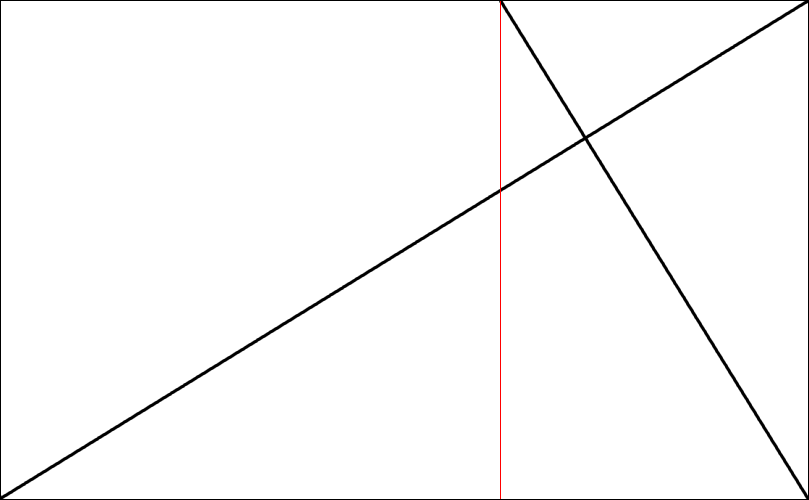
\includegraphics[angle=0,width=0.4\textwidth]{afsnit/fremtidigt_arbejde/billeder/eye_of_god}
    \caption[]{Punktet, hvor de to sorte linjer krydser, kaldes ``The Eye
    of God'', og er her vist i et gyldent rektangel.}
    \label{eye_of_god}
\end{figure}

\begin{figure}[!h]
    \centering
    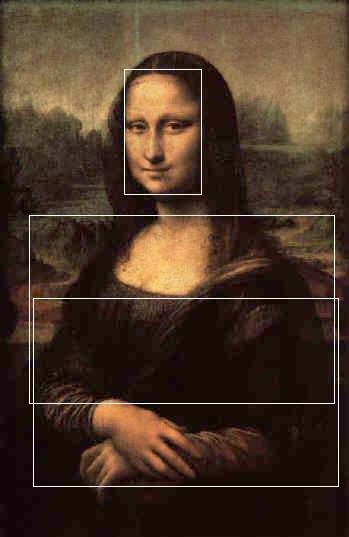
\includegraphics[angle=0,width=0.4\textwidth]{afsnit/fremtidigt_arbejde/billeder/monalisa_fake.jpg}
    \caption[]{Eksempel på regioner i billedet, som er konstrueret i det
    gyldne snit.}
    \label{monalisa_fake}
\end{figure}

\subsection{Udtrækning af regioner}
\begin{itemize}
    \item \textbf{Mere omfattende undersøgelse til fastsættelse af tærskelværdier}\\
        Vente vente. Teste flere billeder. Simpelthen.
    \item \textbf{Automatisk udregning af tærskelværdier}\\
        Med vores nuværende udtrækning af regioner, ville en
        autogenerering af optimale tærskelværdier, for hvert billede,
        være yderst gavnligt for udtrækningen af regioner.
    \item \textbf{Bedre udtrækning af regioner}\\
        Det er oplagt at implementere bedre udtrækning af regioner.
    \item \textbf{Egen, eller bedre, implementation af floodfill}\\
        Den floodfill-metode, som er suppleret af \emph{OpenCV}, giver
        kun areal og afgrænsende rektangel for en farvet region. Vi
        ønsker imidlertid flere informationer om regionen, således at
        det ikke var nødvendigt at approksimere regionen med brug af et
        gitter.
    \item \textbf{Mere sofistikeret valg af tilfældig farve}\\
        Valg af tilfældig farve skal tilpasses således, at vi ikke
        vælger en farve, som ligger indenfor den den tilladte afvigelse.
        Vi vil også gerne undgå at vælge en farve som er i billedet i
        forvejen.
    \item \textbf{Mere målrettet udvælgelse af interessante regioner}\\
        Det kunne være interessant, kun at klassificere regioner som
        interessante, hvis de var et ansigt eller en person.
    \item \textbf{Fuld segmentering af billedet}\\
        I stedet for kun at finde regioner i forhold til et snit i
        billedet, kunne man trække alle regioner ud med det samme. Dette
        vil gøre det lettere, at vurdere regionerne i billedet og man
        vil således også let kunne afgøre om en region lå i flere snit.
\end{itemize}

\subsection{Andre forslag inden for området}
\begin{itemize}
    \item \textbf{Bruge teknikker fra HCI til at finde interessante regioner}\\
        Man kunne gøre brug af \emph{eye tracking} til at finde ud af,
        hvor menneskers øjne fokuserer i malerier. En stor undersøgelse
        kunne da give en indikation af, om der findes nogle objekter,
        eller steder, i malerier, hvor øjnene automatisk drages mod.
\end{itemize}

}

% vim: set tw=72 spell spelllang=da:
